\section{VGG-16}
\subsection{VGG16 là gì}
VGG là viết tắt của Visual Geometry Group; nó là một kiến trúc CNN sâu tiêu chuẩn với nhiều lớp. Kiến trúc VGG là cơ sở của các mô hình nhận dạng đối tượng mang tính đột phá. Được phát triển như một mạng nơ-ron sâu, VGGNet cũng vượt qua các đường cơ sở về nhiều tác vụ và bộ dữ liệu ngoài ImageNet. Hơn nữa, bây giờ nó vẫn là một trong những kiến trúc nhận dạng hình ảnh phổ biến nhất.

Karen Simonyan và Andrew Zisserman \cite{vgg16} đã đề xuất ý tưởng về mạng VGG vào năm 2013 và gửi mô hình thực tế dựa trên ý tưởng này trong ImageNet Challenge 2014. Họ gọi nó là VGG theo tên bộ phận của Visual Geometry Group tại Đại học Oxford nơi họ làm việc.

Mô hình VGG16, hoặc VGGNet, là một mạng nơ-ron phức hợp hỗ trợ 16 lớp. Mô hình VGG16 đạt được độ chính xác gần như 92,7\% trong bài kiểm tra top 5 trong ImageNet (ImageNet là một tập dữ liệu bao gồm hơn 14 triệu hình ảnh thuộc gần 1000 lớp), nó có thể phân loại hình ảnh thành 1000 loại đối tượng, bao gồm bàn phím, động vật, bút chì, chuột, v.v. Ngoài ra, mô hình có kích thước đầu vào hình ảnh là 224 x 224. Nó thay thế các bộ lọc kích thước hạt nhân lớn bằng một số bộ lọc kích thước hạt nhân 3 × 3 lần lượt.

\subsection{Kiến trúc VGG16}
Trong tất cả các cấu hình, VGG16 được xác định là mô hình hoạt động tốt nhất trên tập dữ liệu ImageNet. Hãy xem lại kiến trúc thực tế của cấu hình này (Hình \ref{fig:vgg16_imagenet}).
\begin{figure}[H]
	\centering
	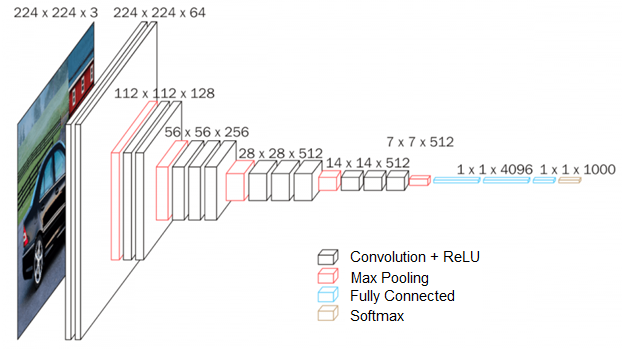
\includegraphics[width=0.6\linewidth]{images/vgg16_imagenet}
	\caption{Kiến trúc VGG16.}
	\label{fig:vgg16_imagenet}
\end{figure}
Đầu vào cho bất kỳ cấu hình mạng nào được coi là hình ảnh có kích thước cố định 224 x 224 với ba kênh R, G và B. Quá trình xử lý trước duy nhất được thực hiện là chuẩn hóa các giá trị RGB cho mỗi pixel. Điều này đạt được bằng cách trừ đi giá trị trung bình cho mỗi pixel.

Hình ảnh được chuyển qua ngăn xếp đầu tiên gồm 2 lớp tích chập có kích thước tiếp nhận rất nhỏ là 3 x 3, tiếp theo là kích hoạt ReLU. Mỗi lớp trong số hai lớp này chứa 64 bộ lọc. Stride được cố định ở 1 pixel và padding là 1 pixel. Cấu hình này bảo toàn độ phân giải không gian và kích thước của bản đồ kích hoạt đầu ra giống với kích thước hình ảnh đầu vào. Các bản đồ kích hoạt sau đó được chuyển qua tổng hợp tối đa không gian trên cửa sổ 2 x 2 pixel, với stride là 2 pixel. Điều này làm giảm một nửa kích thước của các lần kích hoạt. Do đó, kích thước của các kích hoạt ở cuối ngăn xếp đầu tiên là 112 x 112 x 64.

Các kích hoạt sau đó chảy qua ngăn xếp thứ hai tương tự, nhưng với 128 bộ lọc so với 64 bộ lọc trong ngăn xếp thứ nhất. Do đó, kích thước sau ngăn xếp thứ hai trở thành 56 x 56 x 128. Tiếp theo là ngăn xếp thứ ba với ba lớp chập và một lớp tổng hợp tối đa. Số lượng bộ lọc được áp dụng ở đây là 256, làm cho kích thước đầu ra của ngăn xếp là 28 x 28 x 256. Tiếp theo là hai ngăn xếp gồm ba lớp chập, với mỗi ngăn chứa 512 bộ lọc. Đầu ra ở cuối cả hai ngăn xếp này sẽ là 7 x 7 x 512.

Các chồng lớp chập trùng được theo sau bởi ba lớp được kết nối hoàn chỉnh với một lớp làm phẳng ở giữa. Hai lớp đầu tiên có 4.096 tế bào thần kinh mỗi lớp và lớp được kết nối đầy đủ cuối cùng đóng vai trò là lớp đầu ra và có 1.000 tế bào thần kinh tương ứng với 1.000 lớp có thể có cho tập dữ liệu ImageNet. Tiếp theo là lớp đầu ra là lớp kích hoạt Softmax được sử dụng để phân loại (Hình \ref{fig:vgg16_imagenet_detail}).

\begin{figure}[H]
	\centering
	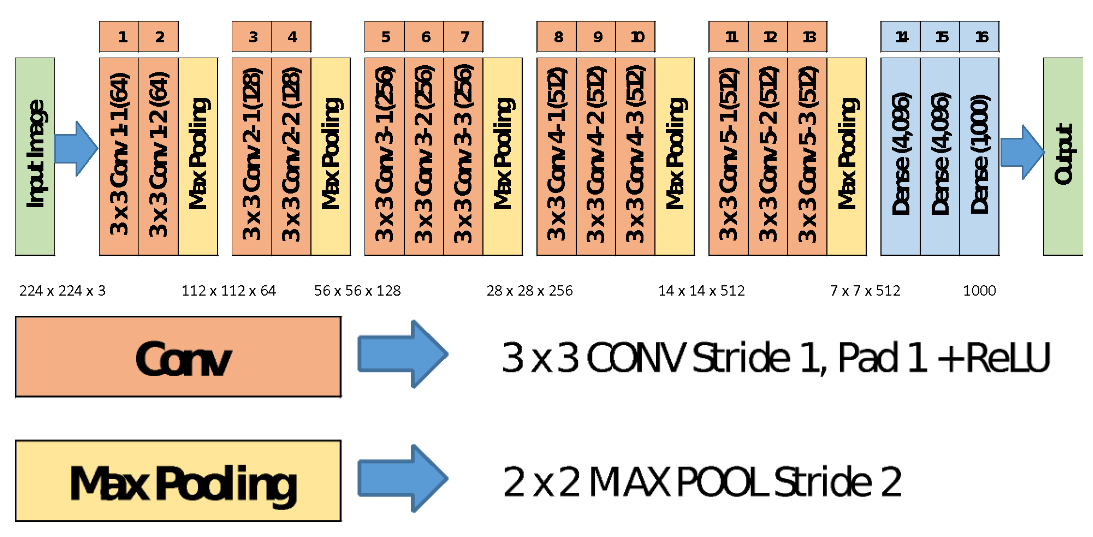
\includegraphics[width=1\linewidth]{images/vgg16_imagenet_detail}
	\caption{Kiến trúc VGG16.}
	\label{fig:vgg16_imagenet_detail}
\end{figure}

\subsection{Trường hợp sử dụng VGG16}
VGG16 khiến các nhà khoa học và nghiên cứu dữ liệu trên toàn thế giới quan tâm mặc dù sự ra đời của nhiều mô hình tính điểm mới và tốt hơn kể từ thời điểm VGG ban đầu được đề xuất. Dưới đây là một số trường hợp sử dụng mà bạn có thể thấy VGG16 được sử dụng thực tế:
\begin{enumerate}
	\item Nhận dạng hoặc phân loại hình ảnh - VGG16 có thể được sử dụng để chẩn đoán bệnh bằng hình ảnh y tế như X-quang hoặc MRI. Nó cũng có thể được sử dụng để nhận biết các biển báo đường phố từ một phương tiện đang di chuyển.
	\item Phát hiện và bản địa hóa hình ảnh - VGG16 có thể hoạt động thực sự tốt trong các trường hợp sử dụng phát hiện hình ảnh. Trên thực tế, nó đã là người chiến thắng trong thử thách phát hiện ImageNet vào năm 2014 (nơi nó kết thúc với vị trí á quân đầu tiên cho thử thách phân loại)
	\item Vectơ nhúng hình ảnh - Sau khi bật ra lớp đầu ra trên cùng, mô hình có thể được sử dụng để đào tạo để tạo vectơ nhúng hình ảnh có thể được sử dụng cho một vấn đề như xác minh khuôn mặt bằng cách sử dụng VGG16 bên trong mạng Siamese.
\end{enumerate}

\subsection{Áp dụng VGG16 vào bài toán của luận văn}
Có hai điểm khác biệt của tập dữ liệu ImageNet và tập dữ liệu được sử dụng trong bài toán của luận văn \cite{dataset} đó là:
\begin{itemize}
	\item Kích thước ảnh đầu vào là 512x512 pixel thay vì 224x224 pixel và ảnh đầu vào là ảnh đa mức xám thay vì ảnh RGB.
	\item Chỉ có 2 lớp đầu ra: Có lao hay không có lao.
\end{itemize}

Điều này dẫn tới 1 chút thay đổi nhỏ trong cấu hình của mô hình VGG16 cho bài toán này (hình \ref{fig:vgg16_luanvan}):
\begin{itemize}
	\item Ảnh đầu vào 512x512x1
	\item Lớp Fully Connected thay đổi lần lượt là 512 và 256
	\item Vì chỉ có 2 lớp đầu ra nên neural đầu ra là 1, hàm kích hoạt là sigmoid. 
\end{itemize}
\begin{figure}[H]
	\centering
	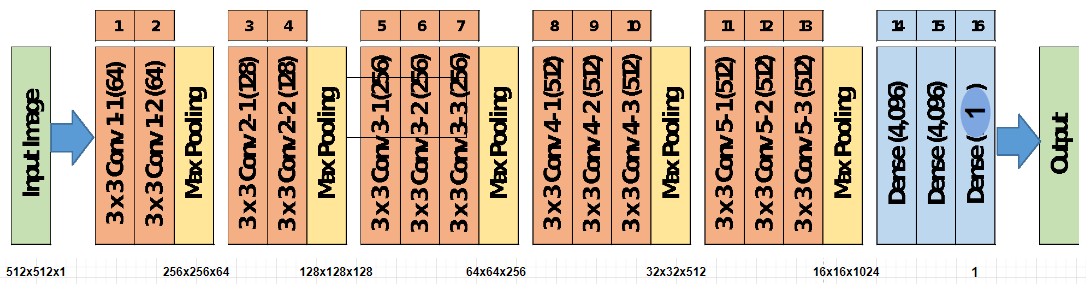
\includegraphics[width=1\linewidth]{images/vgg16_luanvan}
	\caption{Kiến trúc VGG16 cho bài toán của luận văn.}
	\label{fig:vgg16_luanvan}
\end{figure}